
\clearpage
\section{Les transactions}

Dans CUBE PA, la partie 'Transactions' permet de gérer un journal de projet structuré. Le journal de projet regroupe les transactions qui elles regroupent des transactions partielles. Les nombre de transactions partielles est illimité. Pour chaque transaction partielle, CUBE PA met à disposition une chronologie de saisies, avec la saisie la plus récente affichée en haut.

\vspace{\baselineskip}

La philosophie de la structure des transactions et transactions partielles peut être illustrée par l'exemple suivant : Vous êtes promu directeur est vous devez donc vous habiller en conséquence. La transaction 'acheter costumes professionnels' peut être divisée en plusieurs transactions partielles : 'conseil couleur', 'étude de marché des offres en ligne les plus importantes', 'acheter costumes', 'acheter chemises', 'acheter chaussures', etc. Une fois toutes les transactions partielles complétées, la transaction est aussi complétée.

\vspace{\baselineskip}

Un historique est enregistré pour chaque transaction partielle sous forme de saisies. Les saisies correspondent aux lignes d'un fichier Excel. L'idée est d'enregistrer tous les processus relatifs au journal de projet sous forme de saisies. CUBE PA affiche les saisies par ordre chronologique, en commençant par la saisie la plus récente.

\subsection{Créer une transaction}

\begin{wrapfigure}[3]{l}{6.5cm}   % [x] Wie manche Zeile soll sich um die Grafik "brechen"
  \vspace{-35pt}      % Grundwert war 20; mit 30 schön oben beim Text ausgerichtet
  \begin{center}
    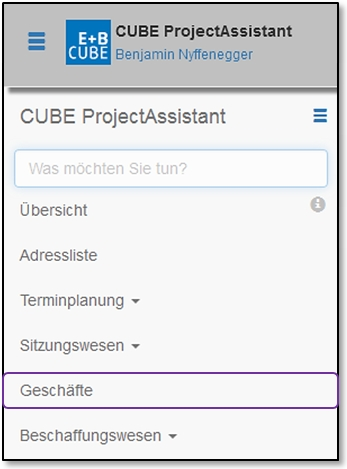
\includegraphics[width=1\linewidth]{../chapters/06_Geschaefte/pictures/6-1_Menu_Geschaefte.jpg}
  \end{center}
  \vspace{-20pt}
  \caption{Organiser les transactions et les contrats}
  \vspace{-10pt}
\end{wrapfigure}

Dans le menu principal à gauche, sélectionnez l'élément 'Transactions'. \\

\vspace{6cm}

\pagebreak

La liste de transactions s'affiche :

\begin{figure}[H]
\center{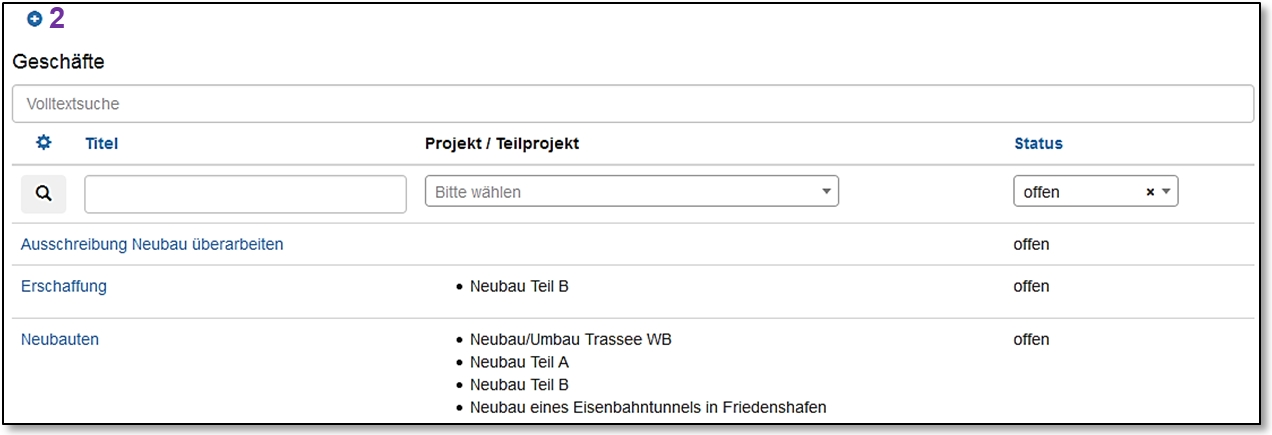
\includegraphics[width=1\linewidth]{../chapters/06_Geschaefte/pictures/6-1_GeschaefteUebersicht.jpg}}
\caption{Aperçu des transactions}
% \label{fig:speciation}
\end{figure}

Cliquez sur le symbole plus (ajouter) 
\includegraphics[height=12pt]{/Icons/Plussymbol.jpg} \col{(2)} en haut à gauche et le masque de saisie d'une nouvelle transaction s'affiche.

\begin{figure}[H]
\center{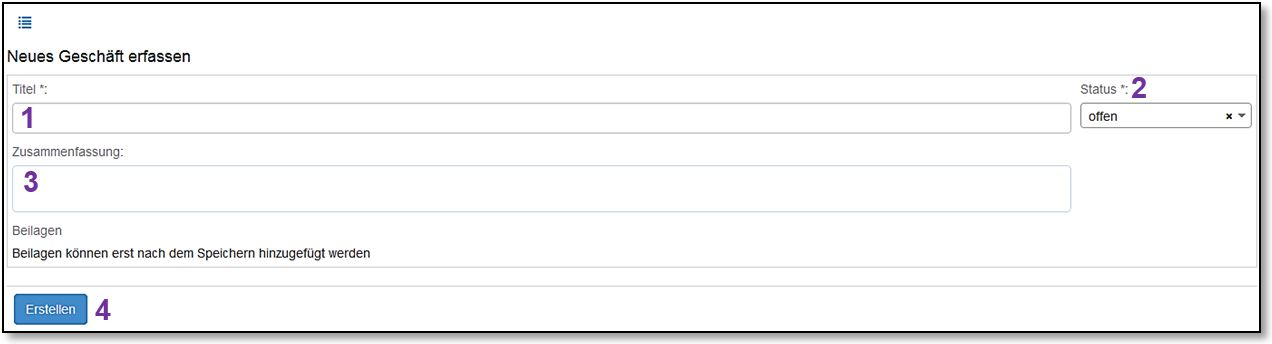
\includegraphics[width=1\linewidth]{61_NeueGeschaefteErfassen.jpg}}
\caption{Saisir une nouvelle transaction}
% \label{fig:speciation}
\end{figure}

Les champs obligatoires sont marqués avec un astérisque (*).

\begin{itemize}
\item
Titre \col{(1)} : Saisissez le titre de la transaction sous forme de texte libre.
\item 
État \col{(2)} : Seuls les deux états 'ouverte' et 'terminée' sont disponibles. Le premier est choisi par défaut lors de la création d'une nouvelle transaction. Le second peut être fixé quand la transaction est terminée.
\item
Résumé \col{(3)} : Décrivez la transaction en quelques lignes de texte libre.
\end{itemize}

Cliquez ensuite sur le bouton 'Créer' 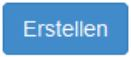
\includegraphics[height=12pt]{/Icons/B_Erstellen.jpg} \col{(4)}. Vous pouvez maintenant charger des pièces jointes.

\begin{figure}[H]
\center{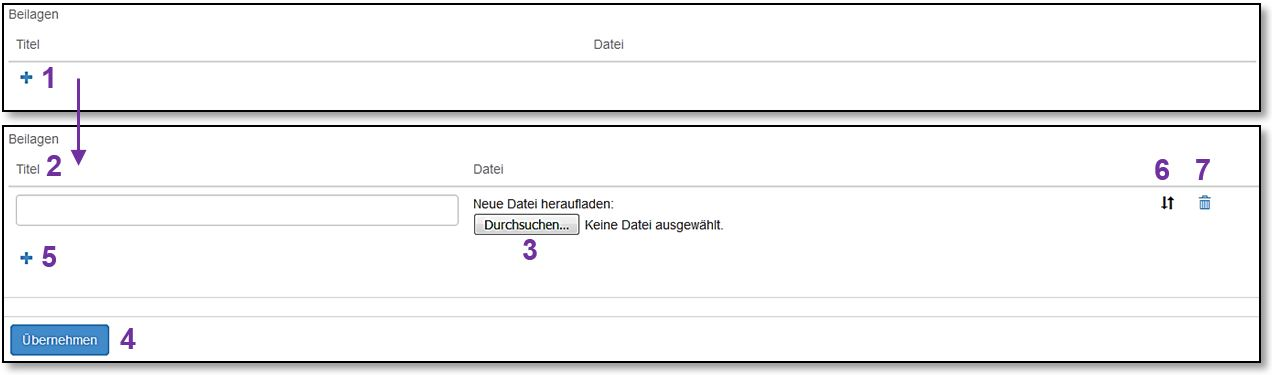
\includegraphics[width=1\linewidth]{61_GeschaefteBeilagenHochladen.jpg}}
\caption{Charger des pièces jointes}
% \label{fig:speciation}
\end{figure}

Le chargement de pièces jointes a pour but d'éviter de saisir des explications trop longues. Vous avez alors la possibilité de faire référence à une pièce jointe.

\vspace{\baselineskip}

Pour ajouter une pièce jointe, cliquez sur le symbole plus (ajouter) 
\includegraphics[height=12pt]{/Icons/Pluszeichen.jpg} \col{(1)}. Les champs pour charger la pièce jointe s'affichent :

\begin{itemize}
\item
Titre \col{(2)} : Saisissez un titre convenable pour la pièce jointe.
\item
Pour charger un document, cliquez sur le bouton de recherche \col{(3)} et double-cliquez sur le fichier désiré. Si vous avez chargé le mauvais fichier, charger simplement un nouveau fichier.
\item
Cliquez ensuite sur le bouton 'Actualiser' \col{(4)} et la pièce jointe est ajoutée.
\end{itemize}


Vous pouvez ajouter autant de pièces jointes que nécessaire en cliquant sur le symbole plus (ajouter) 
\includegraphics[height=12pt]{/Icons/Pluszeichen.jpg} \col{(5)}. Vous pouvez modifier l'ordre des pièces jointes en appuyant sur le symbole avec les deux flèches verticales 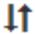
\includegraphics[height=12pt]{/Icons/VertPfeile.jpg} \col{(6)} et en le glissant-déposant à la position voulue. Cliquez sur le symbole de poubelle 
\includegraphics[height=12pt]{/Icons/Muelltonne.jpg} \col{(7)} pour supprimer une pièce jointe.

% bishierher

\subsection{Créer une transaction partielle}

Vous pouvez créer une transaction partielle soit directement dans le même masque où vous avez ajouter des pièces jointes ou en passant à nouveau par le menu et en choisissant l'élément 'Transactions'. Dans la liste de transactions vous pouvez choisir la transaction pour laquelle vous voulez créer une transaction partielle.

\vspace{\baselineskip}

Vous pouvez maintenant visuellement parcourir la liste des transactions ou utiliser la fonction de filtrage. Pour naviguer la liste des transactions, utiliser la pagination en bas de la page. Vous pouvez changer de page en cliquant 'Prochain' et 'Précédent' ou en cliquant sur les numéros de page.

\begin{center}
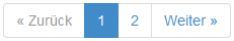
\includegraphics[height=12pt]{/Icons/SeitenBlaettern.jpg}
\end{center}

Vous pouvez utiliser les champs de recherche pour filtrer la liste ou le champ de recherche \col{(1)} pour une recherche plein texte. Dans le champ 'Titre' \col{(2)} vous pouvez saisir du texte libre. Dans le champ 'Projet / Sous-projet' \col{(3)} et le champ 'État' \col{(4)} il y a une liste de sélection. Une fois que vous avez choisi les critères de recherche, cliquez sur le symbole de loupe 
\includegraphics[height=12pt]{/Icons/Lupe_kl.jpg} \col{(5)} à gauche (ou appuyez sur la touche Entrée) et la liste filtrée s'affiche. Vous pouvez alternativement utiliser la recherche plein texte pour chercher des mots clés dans la liste. Cliquez sur le symbole de loupe 
\includegraphics[height=12pt]{/Icons/Lupe_kl.jpg} \col{(5)} ou appuyez la touche Entrée pour lancer la recherche.

\begin{figure}[H]
\center{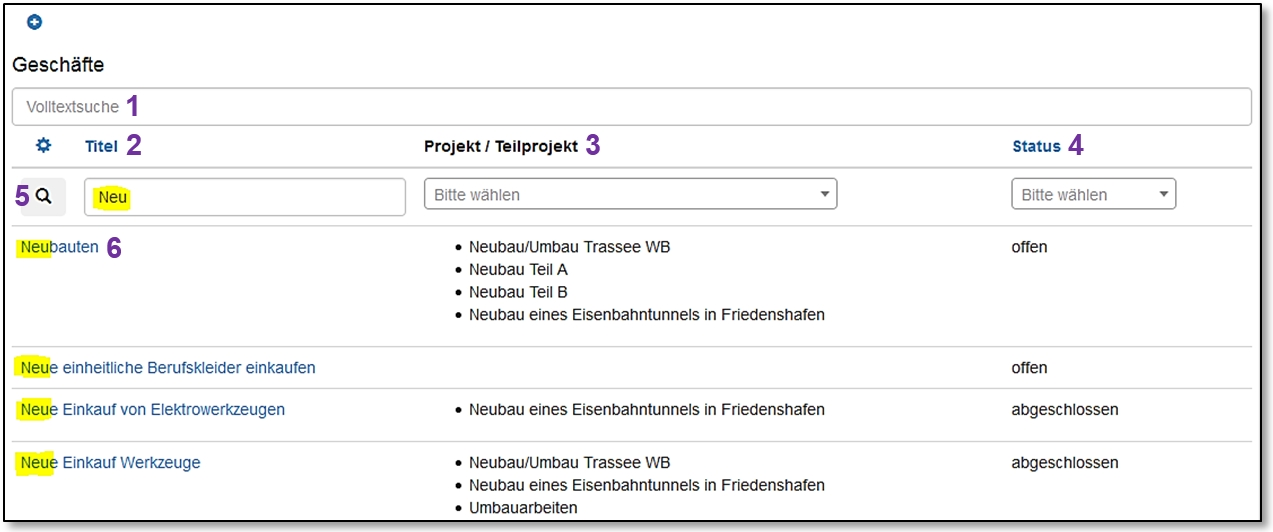
\includegraphics[width=1\linewidth]{../chapters/06_Geschaefte/pictures/6-2_FilterAnwenden.jpg}}
\caption{Utiliser le filtre}
% \label{fig:speciation}
\end{figure}


Quand vous aurez trouvé la transaction recherchée, cliquez sur son titre (bleu) \col{(6)}. Le masque avec l'aperçu de la transaction s'affiche.

\begin{figure}[H]
\center{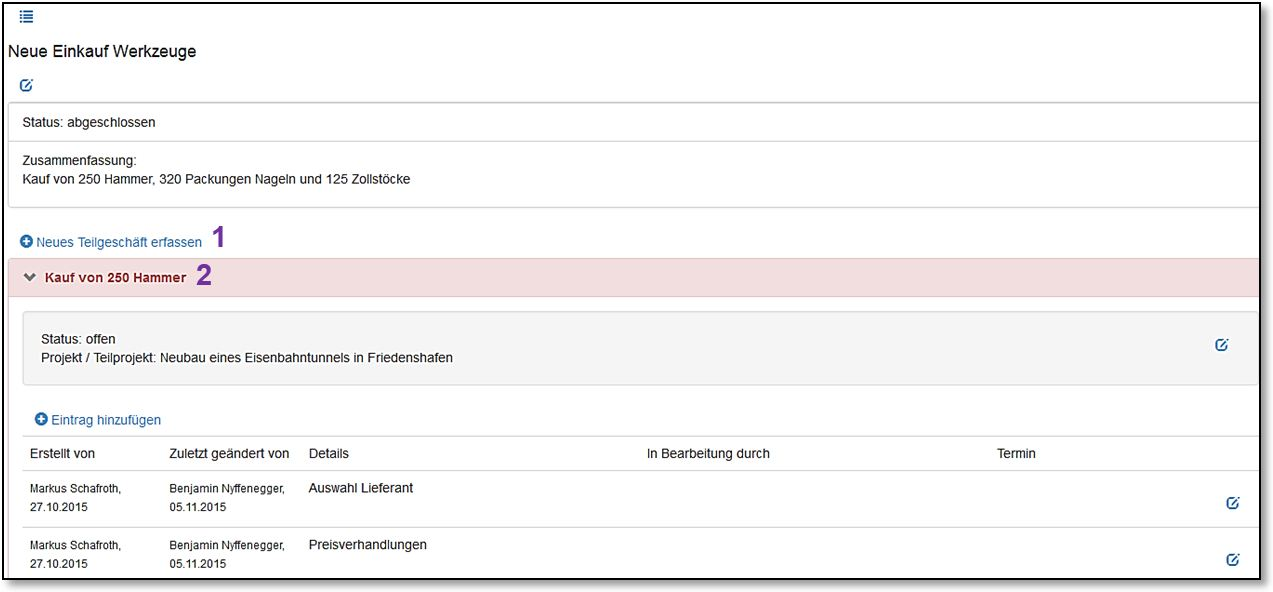
\includegraphics[width=1\linewidth]{62_GeschaefteUebersicht.jpg}}
\caption{Aperçu d'une transaction}
% \label{fig:speciation}
\end{figure}

Sous le titre, l'état, le sommaire, et les pièces jointes vous trouverez un symbole plus (ajouter) 
\includegraphics[height=12pt]{62_TeilgeschaeftErfassen.jpg} \col{(1)} avec lequel vous pouvez créer une nouvelle transaction partielle. Les transactions partielles déjà existantes sont affichées en-dessous \col{(2)}.

\vspace{\baselineskip}

Cliquez sur 'Créer nouvelle transaction partielle' et une fenêtre s'affiche dans laquelle vous pouvez saisir les informations y relatives.

\begin{figure}[H]
\center{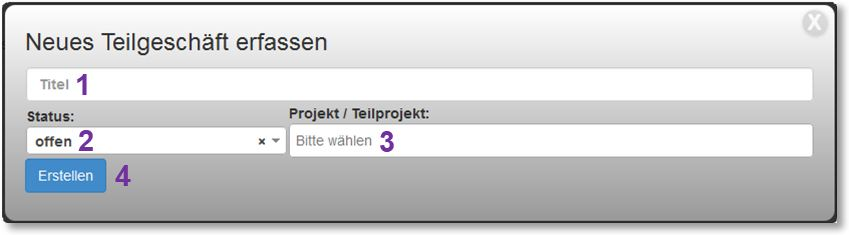
\includegraphics[width=0.5\linewidth]{62_NeuesTeilgeschaeftErfassen.jpg}}
\caption{Créer une nouvelle transaction partielle}
% \label{fig:speciation}
\end{figure}

Saisissez les informations nécessaires dans les champs de saisie :

\begin{itemize}
\item
'Titre' \col{(1)} permet la saisie de texte libre.
\item
'État' \col{(2)} est automatiquement fixé comme 'ouverte'. Quand la transaction partielle est complétée, vous pouvez changer l'état à 'terminée'.
\item
Le champ 'Projet / Sous-projet' \col{(3)} comporte une liste de sélection depuis laquelle vous pouvez lier la transaction partielle à un projet ou à un sous-projet. La transaction à laquelle cette transaction partielle est associée hérite ce lien. Ceci est affiché dans la liste des transactions. La transaction hérite l'ensemble de tous les (sous-)projets liés à ses transactions partielles subordonnées.
\end{itemize}

Cliquez sur le bouton 'Créer' \col{(4)} pour sauvegarder la transaction partielle. Le titre de la transaction partielle apparaît dans le rectangle rose dans l'aperçu de la transaction. Vous pouvez soit ajouter une saisie à la nouvelle transaction partielle soit créer une nouvelle transaction partielle. Si vous créez plusieurs transactions partielles, la dernière que vous avez créée apparaîtra en premier dans l'aperçu.

\subsection{Afficher l'aperçu d'une transaction}

Si vous voulez avoir un aperçu complet d'une transaction, sélectionnez l'élément 'Transactions' dans le menu principal. Cherchez ensuite la transaction pour laquelle vous voulez avoir un aperçu dans la liste des transactions.

\begin{figure}[H]
\center{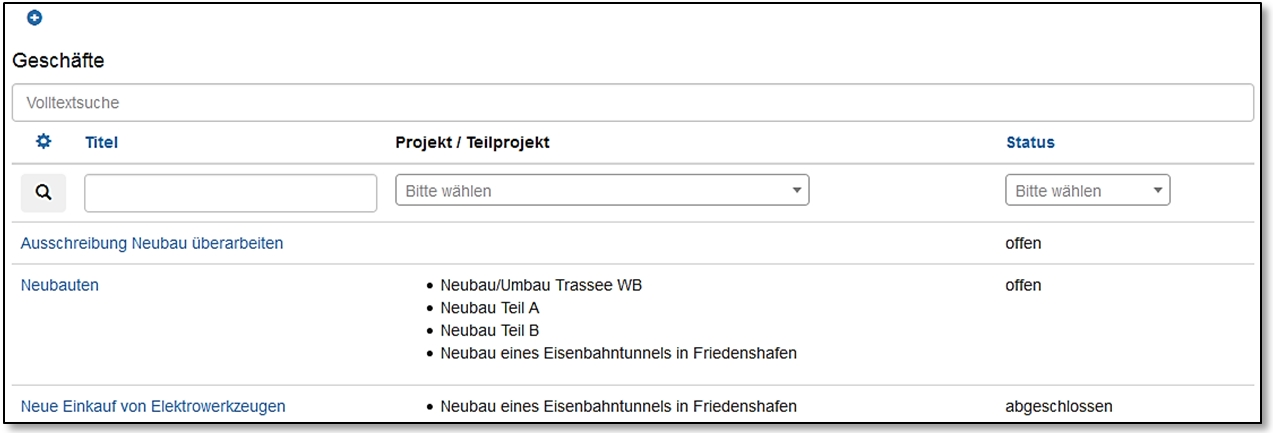
\includegraphics[width=1\linewidth]{../chapters/06_Geschaefte/pictures/6-3_UeberblickGeschaeft.jpg}}
\caption{Aperçu des transactions}
% \label{fig:speciation}
\end{figure}

Vous pouvez maintenant visuellement parcourir la liste des transactions ou utiliser la fonction de filtrage. Pour naviguer la liste des transactions, utiliser la pagination en bas de la page. Vous pouvez changer de page en cliquant 'Prochain' et 'Précédent' ou en cliquant sur les numéros de page.

\begin{center}
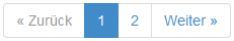
\includegraphics[height=12pt]{/Icons/SeitenBlaettern.jpg}
\end{center}

Vous pouvez utiliser les champs de recherche pour filtrer la liste. Dans le champ 'Titre' \col{(1)} vous pouvez saisir du texte libre. Dans le champ 'Projet / Sous-projet' \col{(2)} et le champ 'État' \col{(3)} il y a une liste de sélection. Une fois que vous avez choisi les critères de recherche, cliquez sur le symbole de loupe 
\includegraphics[height=12pt]{/Icons/Lupe_kl.jpg} \col{(4)} à gauche (ou appuyez sur la touche Entrée) et la liste filtrée s'affiche. Vous pouvez alternativement utiliser la recherche plein texte pour chercher des mots clés dans la liste.

\begin{figure}[H]
\center{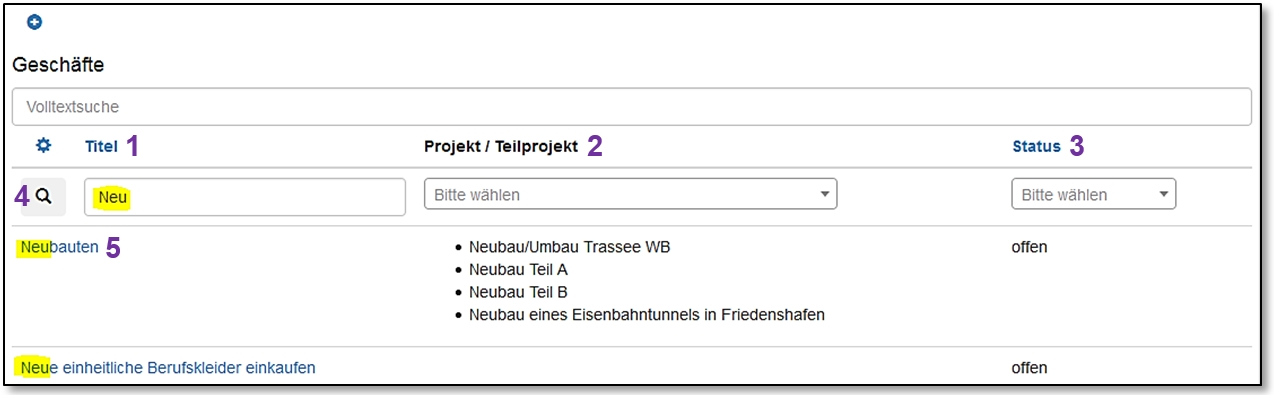
\includegraphics[width=1\linewidth]{../chapters/06_Geschaefte/pictures/6-3_GeschaefteFiltern.jpg}}
\caption{Filtrer les transactions}
% \label{fig:speciation}
\end{figure}

Quand vous aurez trouvé la transaction recherchée, cliquez sur son titre (bleu) \col{(5)}. Le masque avec l'aperçu de la transaction s'affiche.

\begin{figure}[H]
\center{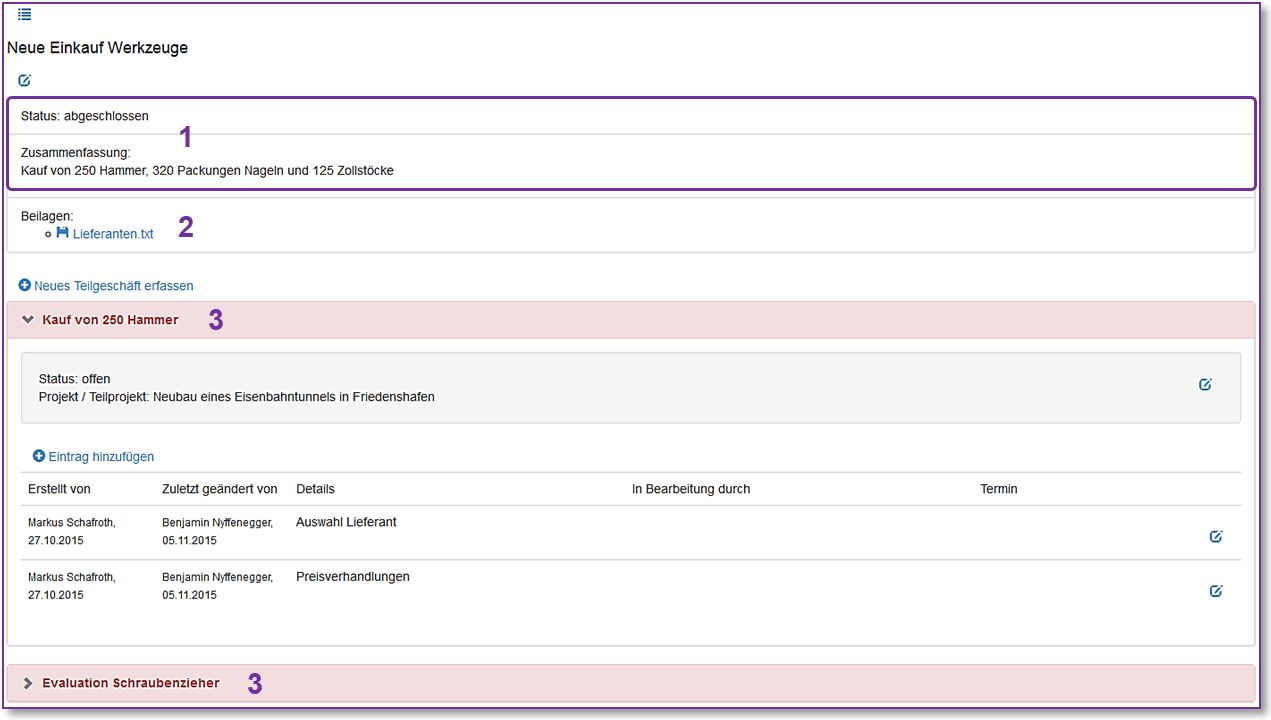
\includegraphics[width=1\linewidth]{63_Geschaeftsuebersicht.jpg}}
\caption{Aperçu d'une transaction}
% \label{fig:speciation}
\end{figure}

Dans cet aperçu vous trouverez les informations générales relatives à cette transaction \col{(1)} et la liste de pièces jointes \col{(2)}, s'il y en a. Plus bas se trouve la liste des transactions partielles \col{(3)}, avec le titre de chacune dans un rectangle rose.

\vspace{\baselineskip}

Choisissez une transaction partielle et cliquez sur la flèche 
\includegraphics[height=12pt]{/Icons/Pfeil_rechts_rosa.jpg} à gauche du titre. La direction de la flèche change d'horizontale en verticale 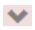
\includegraphics[height=12pt]{/Icons/Pfeil_unten_rosa.jpg} et le contenu de la transaction partielle s'affiche. Les informations générales relatives à la transaction partielle sont affichées en haut, et les saisies sont affichées plus bas, la plus récente en premier.

\vspace{\baselineskip}

Répétez ces étapes pour toutes les transactions partielles et vous aurez un aperçu de toutes les saisies de toutes les transactions partielles de la transaction.

\begin{figure}[H]
\center{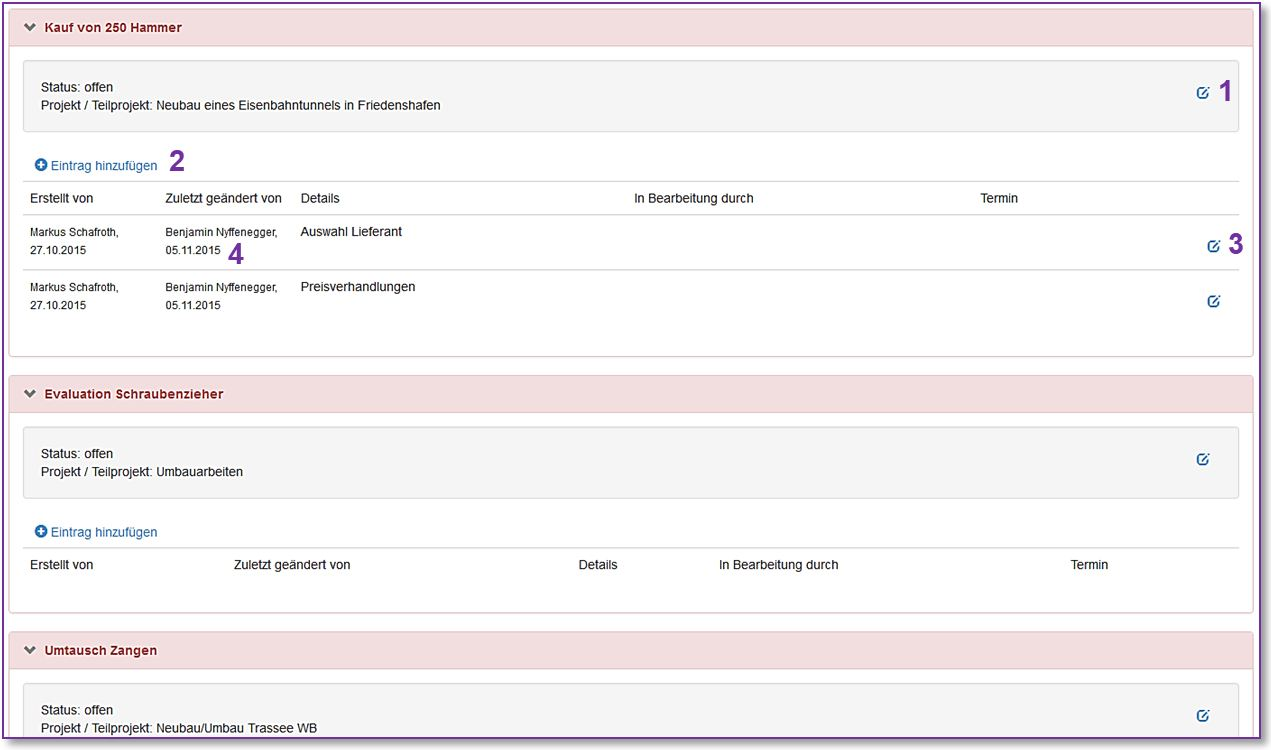
\includegraphics[width=1\linewidth]{63_UeberblickTeilgeschaefte.jpg}}
\caption{Aperçu des transactions partielles}
% \label{fig:speciation}
\end{figure}

Le symbole de crayon 
\includegraphics[height=12pt]{/Icons/Bearbeiten.jpg} \col{(1)} à droite des informations générales d'une transaction partielle vous permet de modifier ces informations.

\subsection{Ajouter des saisies aux transactions partielles}

Vous pouvez ajouter une saisie à une transaction partielle soit directement après l'avoir créée ou plus tard en cherchant la transaction partielle et en affichant son contenu comme mentionné plus haut.

Cliquez sur 'Ajouter saisie' 
\includegraphics[height=12pt]{64_TeilgeschaefteEintragHinzufuegen.jpg} \col{(1)} sous le rectangle gris avec les informations générales relatives à la transaction partielle. La fenêtre pour ajouter une nouvelle saisie s'affiche.

\begin{figure}[H]
\center{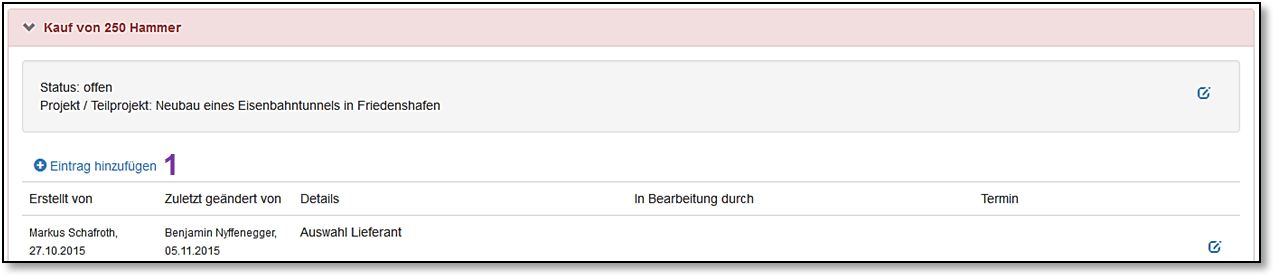
\includegraphics[width=1\linewidth]{64_TeilgeschaefteEintragHinzufuegenMaske.jpg}}
\caption{Aperçu de la transaction partielle}
% \label{fig:speciation}
\end{figure}

\begin{figure}[H]
\center{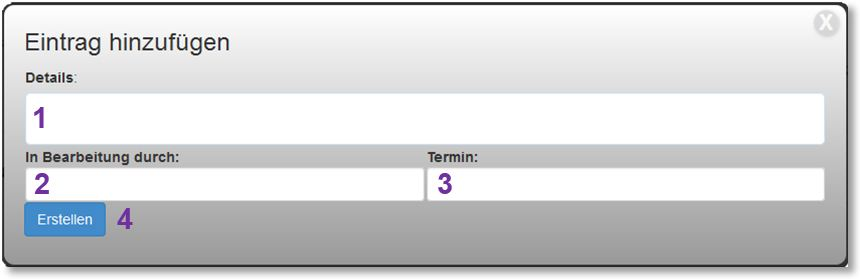
\includegraphics[width=.75\linewidth]{64_TeilgeschaefteHinzufuegenFelder.jpg}}
\caption{Ajouter une nouvelle saisie à une transaction partielle}
% \label{fig:speciation}
\end{figure}

Remplissez les champs de saisie :

\begin{itemize}
\item
'Détails' \col{(1)} est un champ de texte libre pour décrire la saisie (par exemple, la description d'un processus).
\item
'Traité par' \col{(2)} est un champ de texte libre pour saisir qui va traiter la tâche décrite dans la saisie.
\item
'Délai' \col{(3)} est un champ à remplir en format date JJ.MM.AAAA. Il vous permet de préciser quand la tâche décrite dans la saisie doit être accomplie.
\item
Si par exemple la saisie décrit uniquement une constatation, les champs 'Traité par' et 'Délai' ne doivent pas être remplis.
\end{itemize}

Cliquez sur le bouton 'Créer' \col{(4)} et la saisie apparaît dans l'aperçu de la transaction partielle.

\begin{figure}[H]
\center{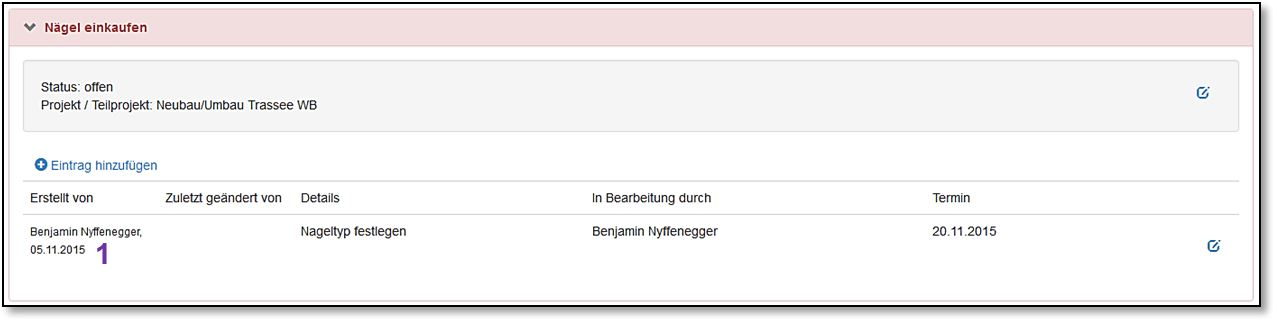
\includegraphics[width=1\linewidth]{64_TeilgeschaeftErstellen.jpg}}
\caption{Aperçu de la transaction partielle}
% \label{fig:speciation}
\end{figure}

A gauche de la saisie, la date de création de la saisie et l'auteur de la saisie \col{(1)} sont visibles. Ceci permet au lecteur de situer cette saisie dans le temps et de poser des questions à propos de la saisie.

Si plusieurs saisies existent pour une même transaction partielle, celles-ci sont affichées en ordre chronologique inverse (la saisie la plus récente en premier).

\subsection{Modifier des saisies existantes}

Pour modifier une saisie existante, affichez d'abord l'aperçu de la transaction concernée et de ses transactions partielles comme décrit plus haut. Affichez les saisies d'une transaction partielle en cliquant sur la flèche 
\includegraphics[height=12pt]{/Icons/Pfeil_rechts_rosa.jpg} à gauche du titre.
	
\begin{figure}[H]
\center{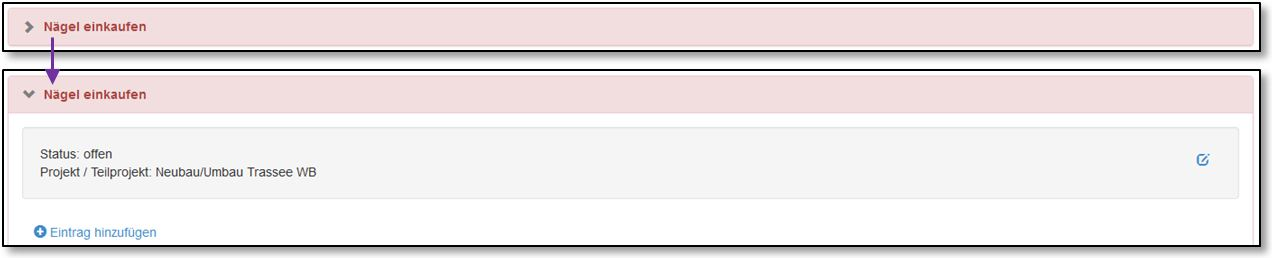
\includegraphics[width=1\linewidth]{65_GeschaefteDetails.jpg}}
\caption{Transactions partielles : Afficher les détails}
% \label{fig:speciation}
\end{figure}

Toutes les saisies de la transaction partielle sélectionnée sont affichées en ordre chronologique inverse (la saisie la plus récente en premier).

\begin{figure}[H]
\center{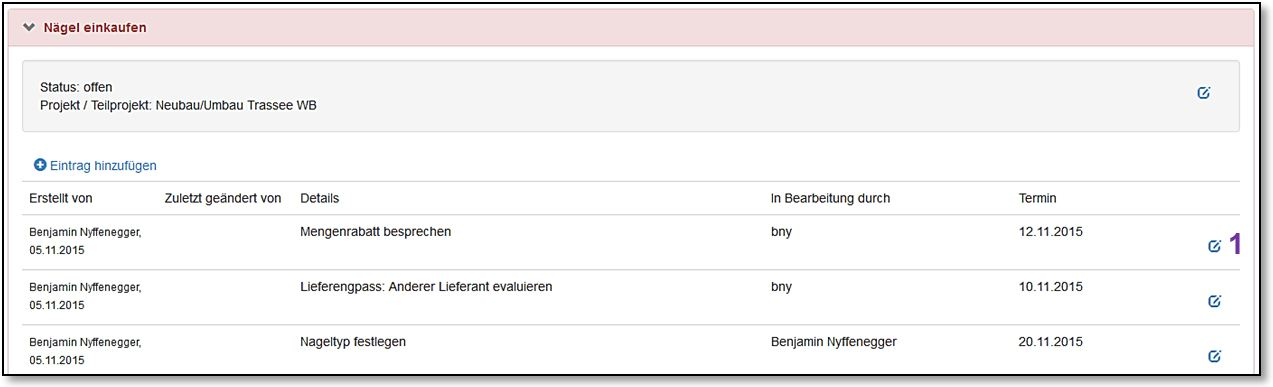
\includegraphics[width=1\linewidth]{65_GeschaefteEintraege.jpg}}
\caption{Transactions partielle : Afficher toutes les saisies}
% \label{fig:speciation}
\end{figure}

Parcourez la liste pour trouver la saisie que vous voulez modifier.

\vspace{\baselineskip}

Cliquez sur le symbole de crayon 
\includegraphics[height=12pt]{/Icons/Bearbeiten.jpg} \col{(1)} à droite de la saisie et la fenêtre pour modifier la saisie s'affiche.

\begin{figure}[H]
\center{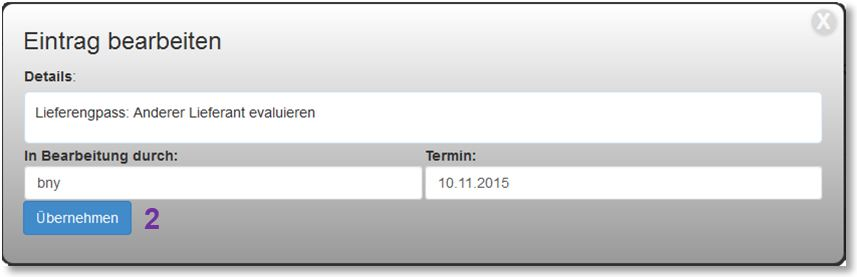
\includegraphics[width=.75\linewidth]{65_GeschaefteEintraegeBearbeiten.jpg}}
\caption{Transactions partielles : Modifier des saisies}
% \label{fig:speciation}
\end{figure}

Modifiez les champs que vous souhaitez modifier et cliquez ensuite sur 'Accepter' \col{(2)}. La saisie modifiée apparaît alors dans la liste des saisies. A gauche, près de la date de création et l'auteur de la saisie, la date de modification de la saisie apparaît avec le nom de l'utilisateur qui a effectué la modification \col{(3)}.

\begin{figure}[H]
\center{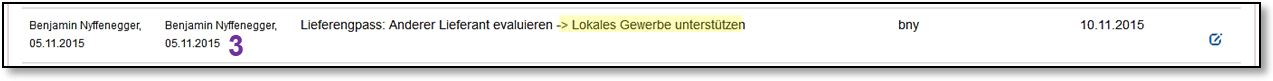
\includegraphics[width=1\linewidth]{65_GeschaefteEintraegeNachverf.jpg}}
\caption{Transactions partielles : Suivre les modifications}
% \label{fig:speciation}
\end{figure}

\textbf{Note} : Le contenu des modifications n'est pas enregistré, c'est-à-dire seul le contenu le plus récent est enregistré.

\vspace{\baselineskip}

\textbf{Note} : Quand une saisie est modifiée plusieurs fois, seuls la date de création, le nom de l'auteur, la date de la dernière modification, et le nom de l'utilisateur qui a fait les dernières modifications sont enregistrés. Les informations relatives aux changements précédents sont perdues.

\subsection{Modifier les informations générales d'une transaction}

Sélectionnez l'élément 'Transactions' dans le menu principal et cherchez la transaction qui vous intéresse dans la liste de transactions, soit en parcourant la liste soit en utilisant la fonction de filtrage. Cliquez sur le titre bleu de la transaction qui vous intéresse. La transaction est ouverte en vue détaillée :

\begin{figure}[H]
\center{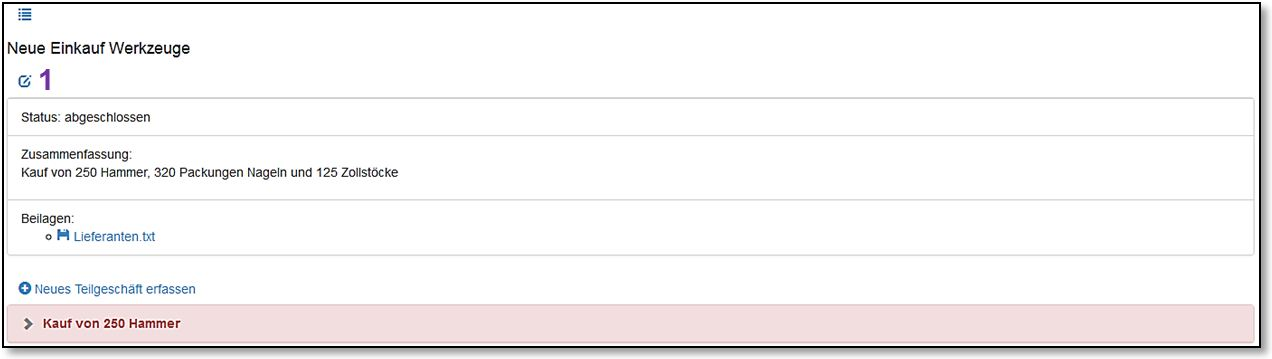
\includegraphics[width=1\linewidth]{66_GeschaefteEintragUeberblick.jpg}}
\caption{Aperçu d'une transaction}
% \label{fig:speciation}
\end{figure}

Cliquez sur le symbole de crayon 
\includegraphics[height=12pt]{/Icons/Bearbeiten.jpg} \col{(1)} sous le titre de la transaction.

\begin{figure}[H]
\center{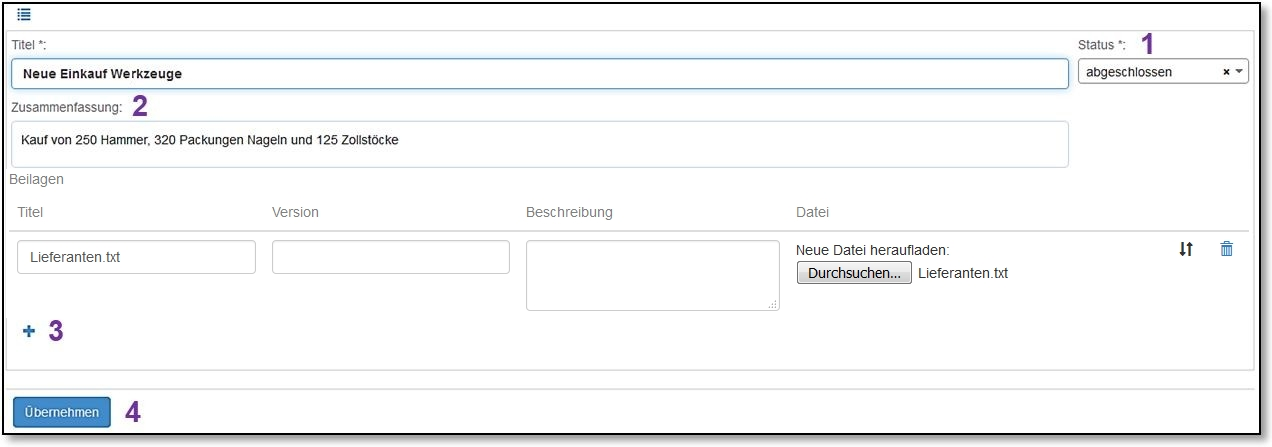
\includegraphics[width=1\linewidth]{../chapters/06_Geschaefte/pictures/6-6_GeschaefteEintragBearbeiten.jpg}}
\caption{Modifier une transaction}
% \label{fig:speciation}
\end{figure}

Vous pouvez modifier le contenu des champs 'État' \col{(1)} et 'Résumé' \col{(2)} et ajouter des pièces jointes \col{(3)}. Cliquez sur 'Accepter' \col{(4)} pour sauvegarder les données.

\subsection{Modifier les informations générales d'une transaction partielle}

Affichez l'aperçu de la transaction qui vous intéresse et de ses transactions partielles correspondantes comme décrit plus haut. Affichez le contenu de la transaction partielle en cliquant sur la flèche 
\includegraphics[height=12pt]{/Icons/Pfeil_rechts_rosa.jpg} à gauche de son titre. Un champ gris \col{(1)} avec les informations générales de la transaction partielle apparaît sous le titre.

\begin{figure}[H]
\center{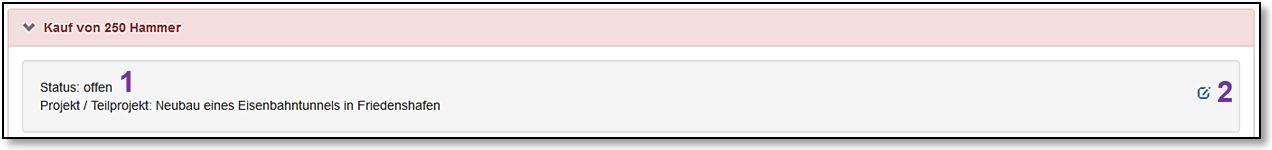
\includegraphics[width=1\linewidth]{67_Teilgeschaeft.jpg}}
\caption{Aperçu d'une transaction partielle}
% \label{fig:speciation}
\end{figure}

Cliquez sur le symbole de crayon 
\includegraphics[height=12pt]{/Icons/Bearbeiten.jpg} \col{(2)} à droite dans ce champ. La fenêtre pour la modification des informations générales de la transaction partielle apparaît.

\begin{figure}[H]
\center{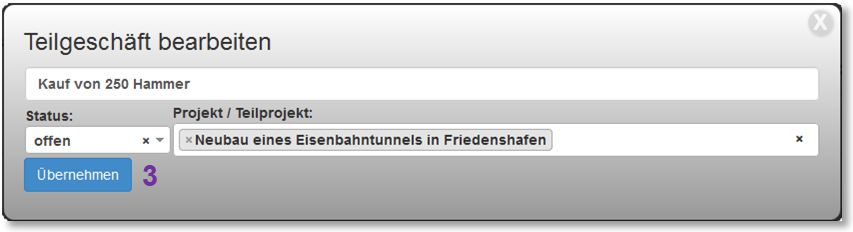
\includegraphics[width=.75\linewidth]{67_TeilgeschaeftBearbeiten.jpg}}
\caption{Modifier une transaction partielle}
% \label{fig:speciation}
\end{figure}

Vous pouvez modifier le contenu des champs. Cliquez ensuite sur 'Accepter' \col{(3)} pour sauvegarder les données.
